\documentclass[journal]{IEEEtran}
\usepackage{graphicx}
\graphicspath{{images/}}

\begin{document}
\title{Explicaci\'on del Controlador ArduinoQuadcopter}
\author{\textit{Ing.} Aldric Ian L\'opez Vergara Anaya }

% The paper headers
\markboth{Ultimo Update ~19 Abril~2015}%
{Shell \MakeLowercase{\textit{et al.}}:Explicacion del Controlador ArduinoQuadcopter}

% make the title area
\maketitle

% Abstract
\begin{abstract}
Este peque\~no art{\'\i}culo tiene la finalidad de documentar y explicar el funcionamiento del proyecto ArduinoQuadcopter. Aunque tambi\'en funciona para otros quads.
\end{abstract}

% Index Terms
\begin{IEEEkeywords}
Control, PID, Aceler\'ometro, Magnet\'ometro, Bar\'ometro, Giroscopio.
\end{IEEEkeywords}

%Introduction
\section{Introducci\'on}
%Primera letra grande y palabra en mayusculas
\IEEEPARstart{E}{n} este art{\'\i}culo se explicara brevemente el funcionamiento del programa para el Arduino Quadcopter. Se explican conceptos de control necesarios as{\'\i} como el uso de distintos sensores del IMU para obtener la posici\'on del sistema. 
\hfill Abril 19, 2015

%Desarrollo
\section{Programa ArduinoQuadcopter}

%Subsecciones
\subsection{Sistema de Control}
El sistema de control  es la parte m\'as importante para que el multirotor pueda volar. A grandes rasgos, el sistema de control son una serie de ecuaciones matem\'aticas que procesa en este caso una peque\~na computadora, llamada microcontrolador, para mantener al veh{\'\i}culo en un vuelo estable.
Cuando el multirotor se encuentra en vuelo, est\'a sometido a muchas fuerzas externas, llamadas perturbaciones, debido al viento, imperfecciones de construcci\'on, etc. Estas perturbaciones pueden hacer que el multirotor no se mantenga estable en el aire. Por ejemplo si nosotros queremos que se mantenga completamente horizontal pero debido a la viento en realidad se termina inclinando levemente, este \'angulo de inclinaci\'on es lo que se conoce en control como error. En general este error se expresa como una simple resta entre el valor deseado y el valor real de la siguiente manera:
\[ e(t)=x_{deseado}(t)-x_{real}(t) \]
En general, el sistema de control intenta minimizar el valor de $e(t)$ para el menor tiempo $t$ posible.
Existen varias estrategias que se pueden tomar para dise\~nar estas ecuaciones que se conocen como algoritmos de control. Dependiendo de la complejidad del sistema que se quiere controlar, en este caso el multirotor, as{\'\i} como de la capacidad de la computadora que se va a utilizar, se elige dicho algoritmo.
En el caso de los multirotores, el algoritmo de control por excelencia es el llamado \textbf{PID}. 

\subsubsection{{?`}Qu\'e es un PID?}
Un \textbf{PID} es un algoritmo de control que combina tres formas del error que se quiere minimizar (la parte proporcional, la integral y la derivativa, por ende el nombre de PID). El \textbf{PID} hace esto mediante una suma de estas tres formas de error asign\'andole un peso espec{\'\i}fico a cada una por medio de tres constantes ($k_p, k_i, k_d$ respectivamente).

\[PID(t)=k_p e(t) + k_i e(t) dt + k_d \frac{d}{dt} e(t)\]

Este valor que se obtiene para PID(t) se le env{\'\i}a al sistema, en este caso al multirotor, por medio de una se\~nal el\'ectrica. El sistema cambia entonces debido a esta se\~nal lo que modifica a su vez el error. El nuevo error es calculado y la computadora se encarga de obtener un nuevo valor para el \textbf{PID} utilizando la ecuaci\'on anterior, completando as{\'\i} el ciclo. 
Generalmente este tipo de controles se expresa mediante un diagrama de bloques:

\begin{figure}[h]
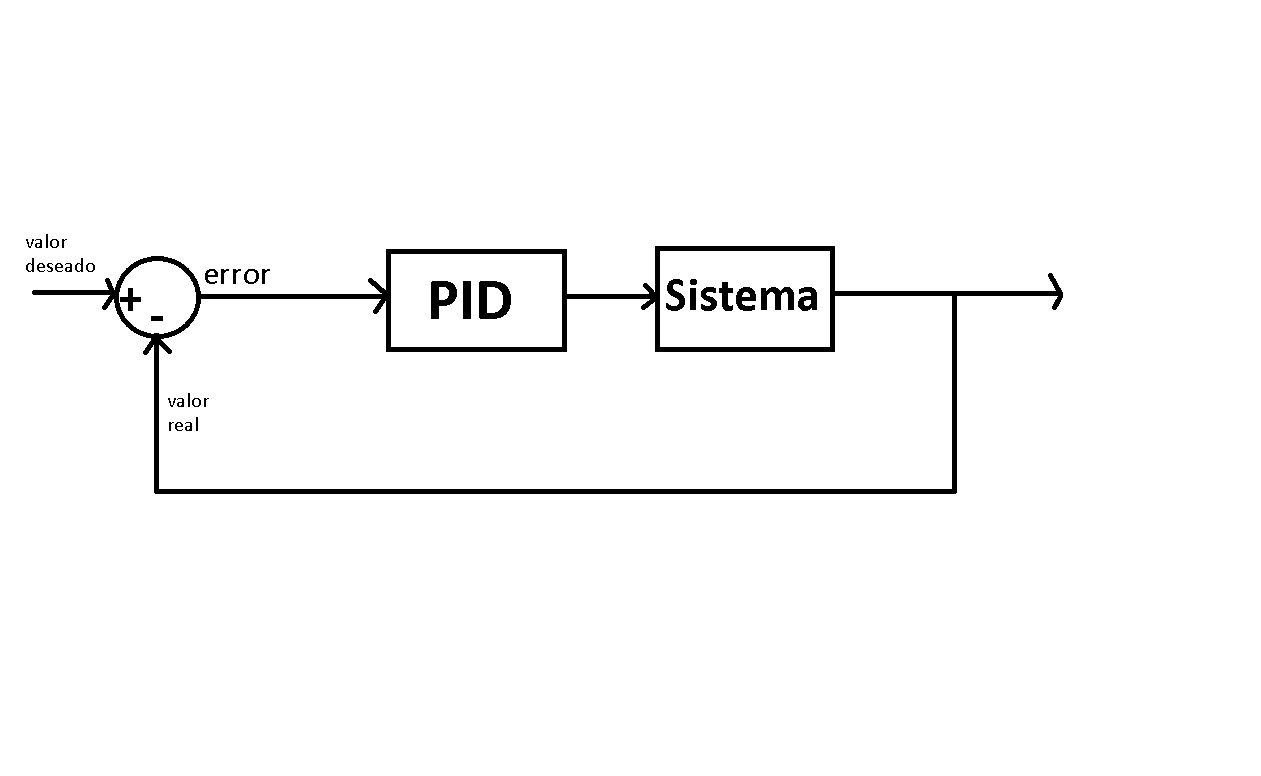
\includegraphics[width=0.5\textwidth]
{PID_explicacion}
\end{figure}

\subsubsection{{?`}Como se aplica el \textbf{PID} al multirotor?}
En el multirotor contamos con actuadores (motores), sensores (aceler\'ometro, giroscopio, magnet\'ometro, bar\'ometro, gps, etc), y un microcontrolador (computadora). Para implementar el control se debe conectar el microcontrolador a los actuadores y sensores. Los sensores le env{\'\i}an al microcontrolador se\~nales el\'ectricas que representan variables f{\'\i}sicas y le permiten encontrar el valor real para calcular el error. Por otro lado los actuadores son la forma que el microcontrolador puede interactuar con el sistema, y son a los que se env{\'\i}a el valor del PID.  
Lo primero que se hace es definir las variables que se quieren controlar, en el caso del multirotor se pueden controlar 3 \'angulos diferentes, as{\'\i} como 3 direcciones espaciales.
En el caso del multirotor es indispensable que la computadora se encargue de controlar los tres \'angulos, ya que un piloto humano no ser{\'\i}a capaz de reaccionar lo suficientemente r\'apido como para corregir los errores. Por otro lado las tres direcciones pueden ser controladas por el piloto \'o en el caso de un multirotor completamente aut\'onomo, mediante controladores \textbf{PID} similares a los que utilicen GPS y bar\'ometro para determinar una posici\'on exacta deseada.
En este caso nos enfocaremos en discutir c\'omo controlar los tres \'angulos de giro, ya que una vez controlados es mucho m\'as sencillo implementar un control para el resto de las direcciones.

\subsection{Midiendo las Variables}
Ahora que sabemos que se van a controlar los tres \'angulos, es importante saber c\'omo medirlos para poder calcular el error. Existen 3 sensores que, combinados, nos permiten hacer dichas mediciones. Estos son: el aceler\'ometro, giroscopio, y magnet\'ometro.
El aceler\'ometro es un sensor que mide la aceleraci\'on neta del multirotor (utilizando una constante acorde al sensor para convertir la se\~nal el\'ectrica a $m/s^{2}$). Si bien parece no ser muy \'util, cuando el multirotor no se esta moviendo, o se mueve a una velocidad estable, la \'unica aceleraci\'on a la que est\'a sometido es debido a la gravedad. Como sabemos que la gravedad es siempre en direcci\'on vertical hacia abajo, es posible calcular mediante trigonometr{\'\i}a el \'angulo en el que se encuentra el multirrotor:

\[\Theta = -\arctan(acc_x acc_y^{2}+acc_z^{2})\]

\[\Gamma = -\arctan(acc_y acc_x^{2}+acc_z^{2})\]

Donde $\Theta$ es el \'angulo hacia $x$ y $\Gamma$ el \'angulo hacia $y$. Para obtener el otro \'angulo, se utiliza otro sensor llamado magnet\'ometro. El magnet\'ometro mide el campo magn\'etico terrestre en las direcciones $x$, $y$, $z$. Si suponemos que el multirotor se encuentra horizontal, el campo magn\'etico \'unicamente est\'a en los ejes $x$, $y$. De esta forma, utilizando trigonometr{\'\i}a nuevamente, se puede conocer, al igual que una br\'ujula, la direcci\'on del norte; y por ende, el \'angulo al que est\'a orientado el multirotor. 

\[\Phi = \arctan(\frac{my}{mx})\]


Por \'ultimo, el giroscopio es un sensor un poco diferente; ya que lo que nos permite medir es la velocidad angular ($\omega$). Es decir, que tan r\'apido o que tan lento est\'a girando sobre alguno de estos ejes. Sin embargo, es posible obtener el \'angulo a partir de esta medici\'on; debido a que la velocidad angular es igual a la derivada con respecto al tiempo del mismo \'angulo.

\[\omega = \frac{d}{dt} \Theta\]


Despejando el \'angulo:

\[\Theta = \int \omega dt\]

Sin embargo, como los microcontroladores que se usan para este tipo de aplicaciones no pueden hacer ni integrales ni derivadas, es necesario aproximar esos valores mediante operaciones m\'as sencillas. En el caso de la integral, se aproxima utilizando el m\'etodo de los rect\'angulos; que no es m\'as que una multiplicaci\'on del tiempo entre dos mediciones, sumada con los valores de \'angulo anteriores.

\[\Theta = \Theta_{anterior} + (t_2-t_1)\omega\]


Esto se puede aplicar para los tres \'angulos respectivamente, por lo que ahora se tienen dos mediciones de sensores diferentes para cada \'angulo. 

Finalmente, se deben combinar estas mediciones. Es importante juntar dos sensores para cada uno de los \'angulos, ya que cada sensor tiene una mayor o menor confiabilidad dependiendo de las condiciones. En el caso del aceler\'ometro y del magnet\'ometro, funcionan mejor cuando la velocidad angular es cercana a cero; es decir, que los \'angulos no cambian muy r\'apidamente. Por otro lado, el giroscopio, al ser un medidor de velocidades angulares, funciona mejor cuando los \'angulos cambian r\'apidamente; pero muy malo para cuando las velocidades angulares son cercanas a cero. 
Los sensores se combinan entonces utilizando un filtro complementario de la siguiente forma:

\[\Theta =\alpha (\Theta_{anterior}+\omega_{\Theta_{giro}} (t_2-t_1))+(1-\alpha)\Theta_{acel}\]

\[\Gamma =\alpha (\Gamma_{anterior}+\omega_{\Gamma_{giro}} (t_2-t_1))+(1-\alpha)\Gamma_{acel}\]

\[\Phi =\alpha (\Phi_{anterior}+\omega_{\Phi_{giro}} (t_2-t_1))+(1-\alpha)\Phi_{acel}\]

Donde $\alpha$ es una constante entre 0 y 1 que nos indica la confiabilidad que se tiene para cada medici\'on. Esta constante depende de la combinaci\'on de sensores que se utiliza para cada medici\'on. En este caso es preferible tener una  con valores altos (usualmente entre 0.85 y 0.99) de forma tal que se conf{\'\i}e m\'as en el giroscopio cuando haya velocidades angulares grandes y menos cuando sean peque\~nas.
Estos valores para los tres \'angulos son los que ahora se env{\'\i}an como retroalimentaci\'on de valor real para calcular el error del PID.

\subsection{Implementando el PID}
La ecuaci\'on del \textbf{PID} es una ecuaci\'on integro-diferencial; es decir, que incluye tanto integrales como derivadas. Por lo que es necesario reemplazarlas por aproximaciones discretas. En este caso se pueden utilizar aproximaci\'on de rect\'angulos para las integrales, y diferencias para las derivadas. Por lo que la ecuaci\'on de PID:


\[PID(t)=k_p e(t) + k_i \int e(t) dt + k_d \frac{d}{dt} e(t)\]

Se convierte en:


\[PID(n)=k_p e(n) + k_i e(n) (t_n-t_{n-1})+I_{anterior} + k_d \frac{e(n)-e(n-1)}{t_n-t_{n-1}} \]

Donde $I_{anterior}$ se calcula a partir de la parte integral

\[I_{anterior}=k_i e(n) (t_n-t_{n-1})+I_{anterior}\]

De esta manera se completa el ciclo del PID; ahora resta solamente aplicarlo a cada uno de los \'angulos. Para esto nos interesa controlar dos aspectos de cada eje de giro: el \'angulo de inclinaci\'on en s{\'\i} y  la velocidad angular del mismo eje. Esto se logra utilizando dos controladores \textbf{PID}  por cada eje mediante etapas como se puede ver en el diagrama con mayor facilidad:

\begin{figure}[h]
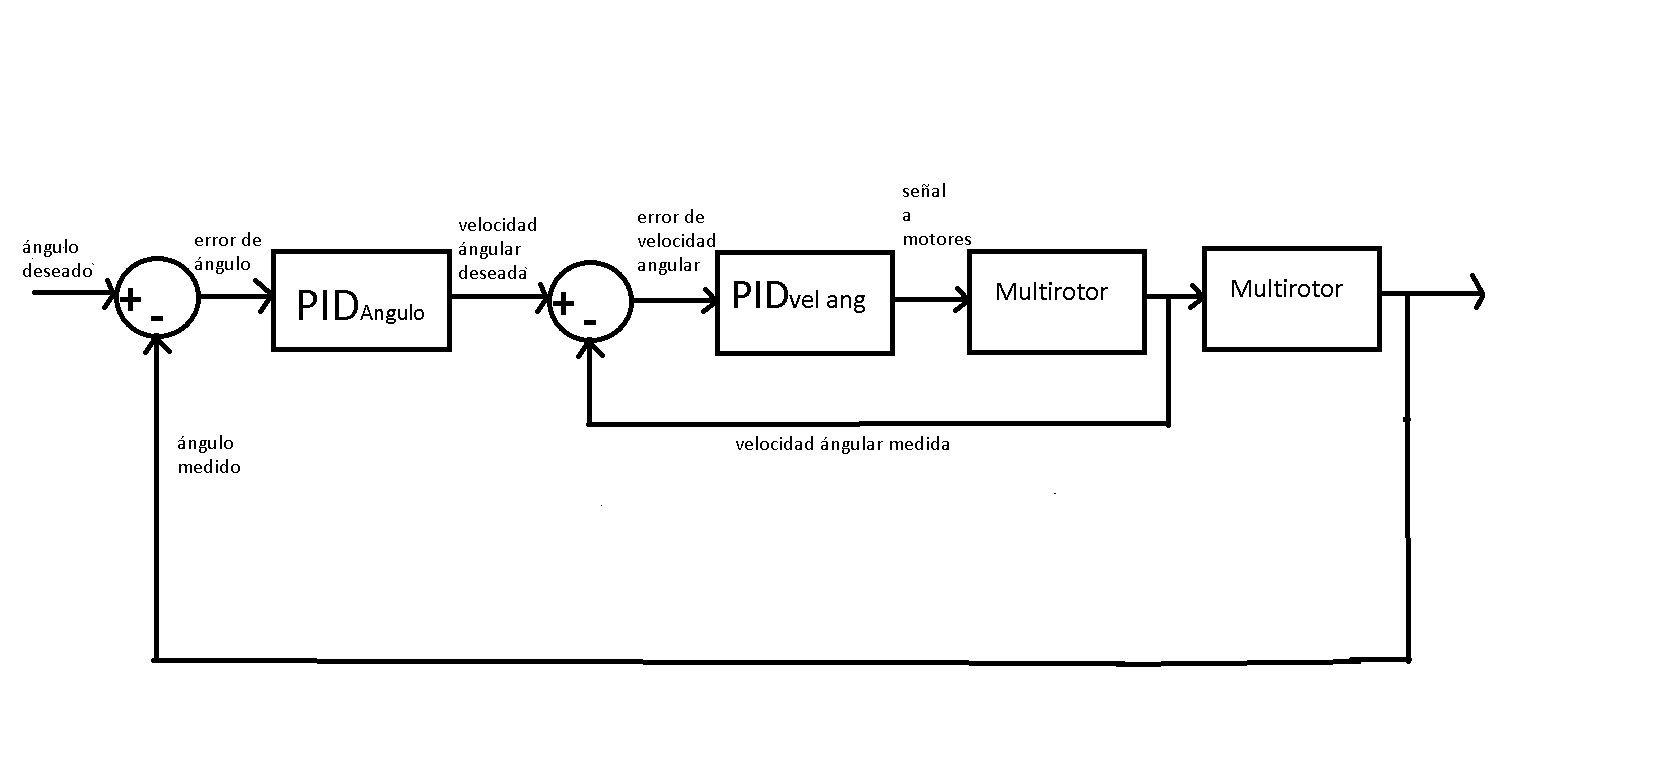
\includegraphics[width=0.5\textwidth]
{PID_explicacion_Completa}
\end{figure}

Estos dos \textbf{PID} anidados nos permiten controlar ambas variables al mismo tiempo para cada \'angulo de manera individual, tomando la retroalimentaci\'on de la velocidad angular directamente del giroscopio, y la retroalimentaci\'on del \'angulo del filtro complementario que se explic\'o previamente. 

Por \'ultimo, se deben combinar todas las se\~nales a los motores de forma tal que controlen en conjunto el multirotor. Esto depende de la configuraci\'on en que se encuentren los motores; ya que en algunos, esta se\~nal ser\'a positiva y en otros negativa. Para el ejemplo de un multirotor quadc\'optero en configuraci\'on X las se\~nales ser{\'\i}an:

\[MotoresPWM_0=throttle+PID_{roll}-PID_{pitch} -PID_{yaw}\]
\[MotoresPWM_1=throttle-PID_{roll}-PID_{pitch} +PID_{yaw}\]
\[MotoresPWM_2=throttle-PID_{roll}+PID_{pitch} -PID_{yaw}\]
\[MotoresPWM_3=throttle+PID_{roll}+PID_{pitch} +PID_{yaw}\]

\subsection{Sintonizaci\'on}

Con todas estas ecuaciones listas, se puede programar al microcontrolador el c\'odigo para el algoritmo de control. Lo \'unico que resta es la sintonizaci\'on del PID. Esto se refiere a encontrar los valores de las tres constantes $k_p$, $k_i$, $k_d$, para cada uno de los controladores. 
Existe una rama importante de la ingenier{\'\i}a que estudia la manera de encontrar dichas constantes que se conoce como teor{\'\i}a de control. Mediante modelos matem\'aticos y distintos criterios de estabilizaci\'on se pueden encontrar los mejores valores para el PID.
Sin embargo, existen algoritmos m\'as sencillos que permiten encontrar estas constantes mediante experimentaci\'on, utilizando prueba y error. Se eligen primero valores de $k_i$ y $k_d$ muy cercanos a cero. Despu\'es se incrementa el valor de $k_p$ hasta que el multirotor comienza a oscilar, entonces se decrementa ligeramente el valor de $k_p$.
El tipo de respuesta que se busca es cr{\'\i}ticamente amortiguado, que es el m\'as r\'apido. Si oscila puede estar sobre amortiguado, en cuyo caso $k_p$ debe reducirse, o subamortiguado, $k_p$ debe incrementarse.

Despu\'es, se incrementan gradualmente los valores de $k_i$ y $k_d$ de acuerdo a la respuesta que se obtenga y que se quiera lograr. La constante $k_i$ permite eliminar el error en estado estable, mientras que $k_d$ permite acelerar la velocidad a la que el controlador responde. Esta forma de encontrar las constantes si bien requiere de mayor tiempo y experiencia, es la forma m\'as sencilla de hacerlo.  

De esta forma, es posible ahora enviar un \'angulo deseado al microcontrolador, y este se encargar\'a de que el multirotor se mantenga en ese \'angulo mientras nosotros lo deseemos, y as{\'\i} moverse en cualquier direcci\'on, o mantenerse est\'atico. Para controlar la posici\'on de forma autom\'atica se puede incluir otro \textbf{PID} con retroalimentaci\'on de GPS y bar\'ometro que tenga como salida el \'angulo de inclinaci\'on del multirotor.

%Conclusion
\section{Conclusi\'on}
El resultado de este algoritmo puede verse en el programa de Arduino.

%Apendices
%\appendices
%\section{Titulo Appendice A}
%Appendix one text goes here.

%Referencias
%\begin{thebibliography}{1}
%\bibitem{Cita1}
%El.~Apellido, \emph{Titulo del libro}, 1ra~ed.\hs$k_i$p 1em plus
%  0.5em minus 0.4em\relax DF, Mexico: Editorial, 1992.
%\end{thebibliography}

%Final
\end{document}